% exercise sheet with header on every page for math or close subjects
\documentclass[12pt]{article}
\usepackage[utf8]{inputenc}
\usepackage{latexsym}
\usepackage{multicol}
\usepackage{fancyhdr}
\usepackage{amsfonts}
\usepackage{amsmath}
\usepackage{amssymb}
\usepackage{enumerate}
\usepackage{listings}
\usepackage{graphicx}

% Shortcuts for bb, frak and cal letters
\newcommand{\E}{\mathbb{E}}
\newcommand{\V}{\mathbb{V}}
\renewcommand{\P}{\mathbb{P}}
\newcommand{\N}{\mathbb{N}}
\newcommand{\R}{\mathbb{R}}
\newcommand{\C}{\mathbb{C}}
\newcommand{\Z}{\mathbb{Z}}
\newcommand{\Pfrak}{\mathfrak{P}}
\newcommand{\Pfrac}{\mathfrak{P}}
\newcommand{\Bfrac}{\mathfrak{P}}
\newcommand{\Bfrak}{\mathfrak{B}}
\newcommand{\Fcal}{\mathcal{F}}
\newcommand{\Ycal}{\mathcal{Y}}
\newcommand{\Bcal}{\mathcal{B}}
\newcommand{\Acal}{\mathcal{A}}

% formating
\topmargin -3.5cm
\textheight 22cm
\textwidth 16.0 cm
\oddsidemargin -0.1cm

% Fancy Header on every Page
\pagestyle{fancy}
\lhead{\textbf{Embedded Systems Milestone 1}}
\rhead{Daniel Schäfer (2549458)\\ Rafael Dewes (2548365)\\ Kevin M\"uller (2550062)}
\renewcommand{\headrulewidth}{1.2pt}
\setlength{\headheight}{110pt}

\begin{document}
\pagenumbering{gobble}
\lstset{language=C++}

\section*{Pins}

\subsection*{Scout}

\small
\begin{tabular}{c || p{30mm} | p{30mm} | p{60mm}}
  \hline
  \textbf{PIN} & FUNCTION & alternate Functions & NOTES\\
  \hline
  \hline
  \hline
  \textbf{PB4} & LCD data line DB5 & User push button,\newline ISP Programming line & Push buttons with inverted logic!\newline PB4 (PCINT4) can also serve as an internal interrupt source\\
  \hline
  \textbf{PB5} & LCD data line DB6 & User push button,\newline ISP Programming line & Push buttons with inverted logic!\newline PB5 (PCINT5) can also serve as an internal interrupt source\\
  \hline
  \textbf{PB0} & LCD Control Line R/W & Timer1 input capture (ICP1),\newline divided system clock output (CLK0) & \\
  \hline
  \textbf{PD4} & LCD control line E & USART external clock input/output (XCK)\newline Timer0 external counter (T0) & \\
  \hline
  \textbf{PD7} & LCD data line DB7 & connected to green user LED & high value turns LED on\\
  \hline
  \textbf{PD2} & LCD control line RS & external interrupt 0 (INT0) & NOTE\\
  \hline
  \textbf{PB1} & LCD data line DB4 & user pushbutton,\newline Timer1 PWM output A (OC1A) & inverted logic on button\\
  \hline
  \textbf{PC5} & analog input and digital I/O & jumpered to sensors IR LEDs (driving low turns off emitters),\newline ADC input channel 5 (ADC5) & \\
  \hline
  \textbf{PD0} & free digital I/O & USART input pin (RXD) & DEV port RX\\
  \hline
  \textbf{PD1} & free digital I/O & connected to red user LED,\newline USART input pin (TXD) & DEV port TX\\
  \hline
\end{tabular}
\normalsize


\subsection*{Collector} 
\small 
\begin{tabular}{c || p{30mm} | p{30mm} | p{60mm}}
  \hline
  \textbf{PIN} & FUNCTION & alternate Functions & NOTES\\
  \hline
  \textbf{PB0} & Red LED (RX)\newline User pushbutton C\newline LCD data line DB5 & SPI slave select ($\overline{\text{SS}}$)\newline Pin-change interrupt (PCINT0) & \\
  \hline
  \textbf{PD5} & Green LED (TX)\newline
User pushbutton B\newline
LCD data line DB7 \newline & UART external clock (XCK1)\newline
UART flow control ($\overline{\text{CTS}}$) & \\
  \hline
  \textbf{PD7} & Buzzer PWM & Analog input (ADC10)\newline Timer4 PWM output D (OC4D)\newline Timer0 counter source (T0) & \\
  \hline
  \textbf{PB3} & User pushbutton A\newline LCD data line DB4  & SPI Master Input/Slave Output (MISO)\newline Pin-change interrupt (PCINT3)  & Push buttons with inverted logic!\\
  \hline
  \textbf{PC7} & Yellow LED\newline LCD data line DB6 & Timer4 PWM output A (OC4A)\newline Timer3 input capture pin (ICP3)\newline Divided system clock output (CLKO) & \\
  \hline
  \textbf{PD2} & LCD control line (RS) & UART receive pin (RXD1)\newline External interrupt source ($\overline{\text{INT2}}$) & \\
  \hline
  \textbf{PD3} & LCD control line (E) & UART transmit pin (TXD1)\newline External interrupt source ($\overline{\text{INT3}}$) & \\
\end{tabular}
\normalsize

\section*{Interrupts}

\section*{Hybrid Automata}
\subsection* {Scout}
The scout has two modes of operation: Moving in the dark (areas with photo sensor readings \leq 200) and light areas (areas with photo sensor readings > 200). The input sensor readings are in the variable photoSignal. In both states, position and angles are modelled as derivates of the left and right angular wheel velocities u\textsubscript{l} and u\textsubscript{r}. For simplicity, we modelled the wheels in a way that they can either turn forward or backward with constant speed of 1. We also introduced continuous variables for the harvesting positions which are only updated in the state MoveInLight. Before that, they remain at -1. Those variables as well as the angular wheel velocities are also the output variables. The self-loop in MoveInLight updates the variable bestP with the best photo sensor reading so far. From the exercise we were not sure whether this best value should only include values > 200 or all values. If we would want all values we would have to add such a self-loop in the MoveInDark state. Another continuous variable clock keeps track of the time and triggers a transition to state Done after 300 seconds where the best harvesting position read so far will be output.\\
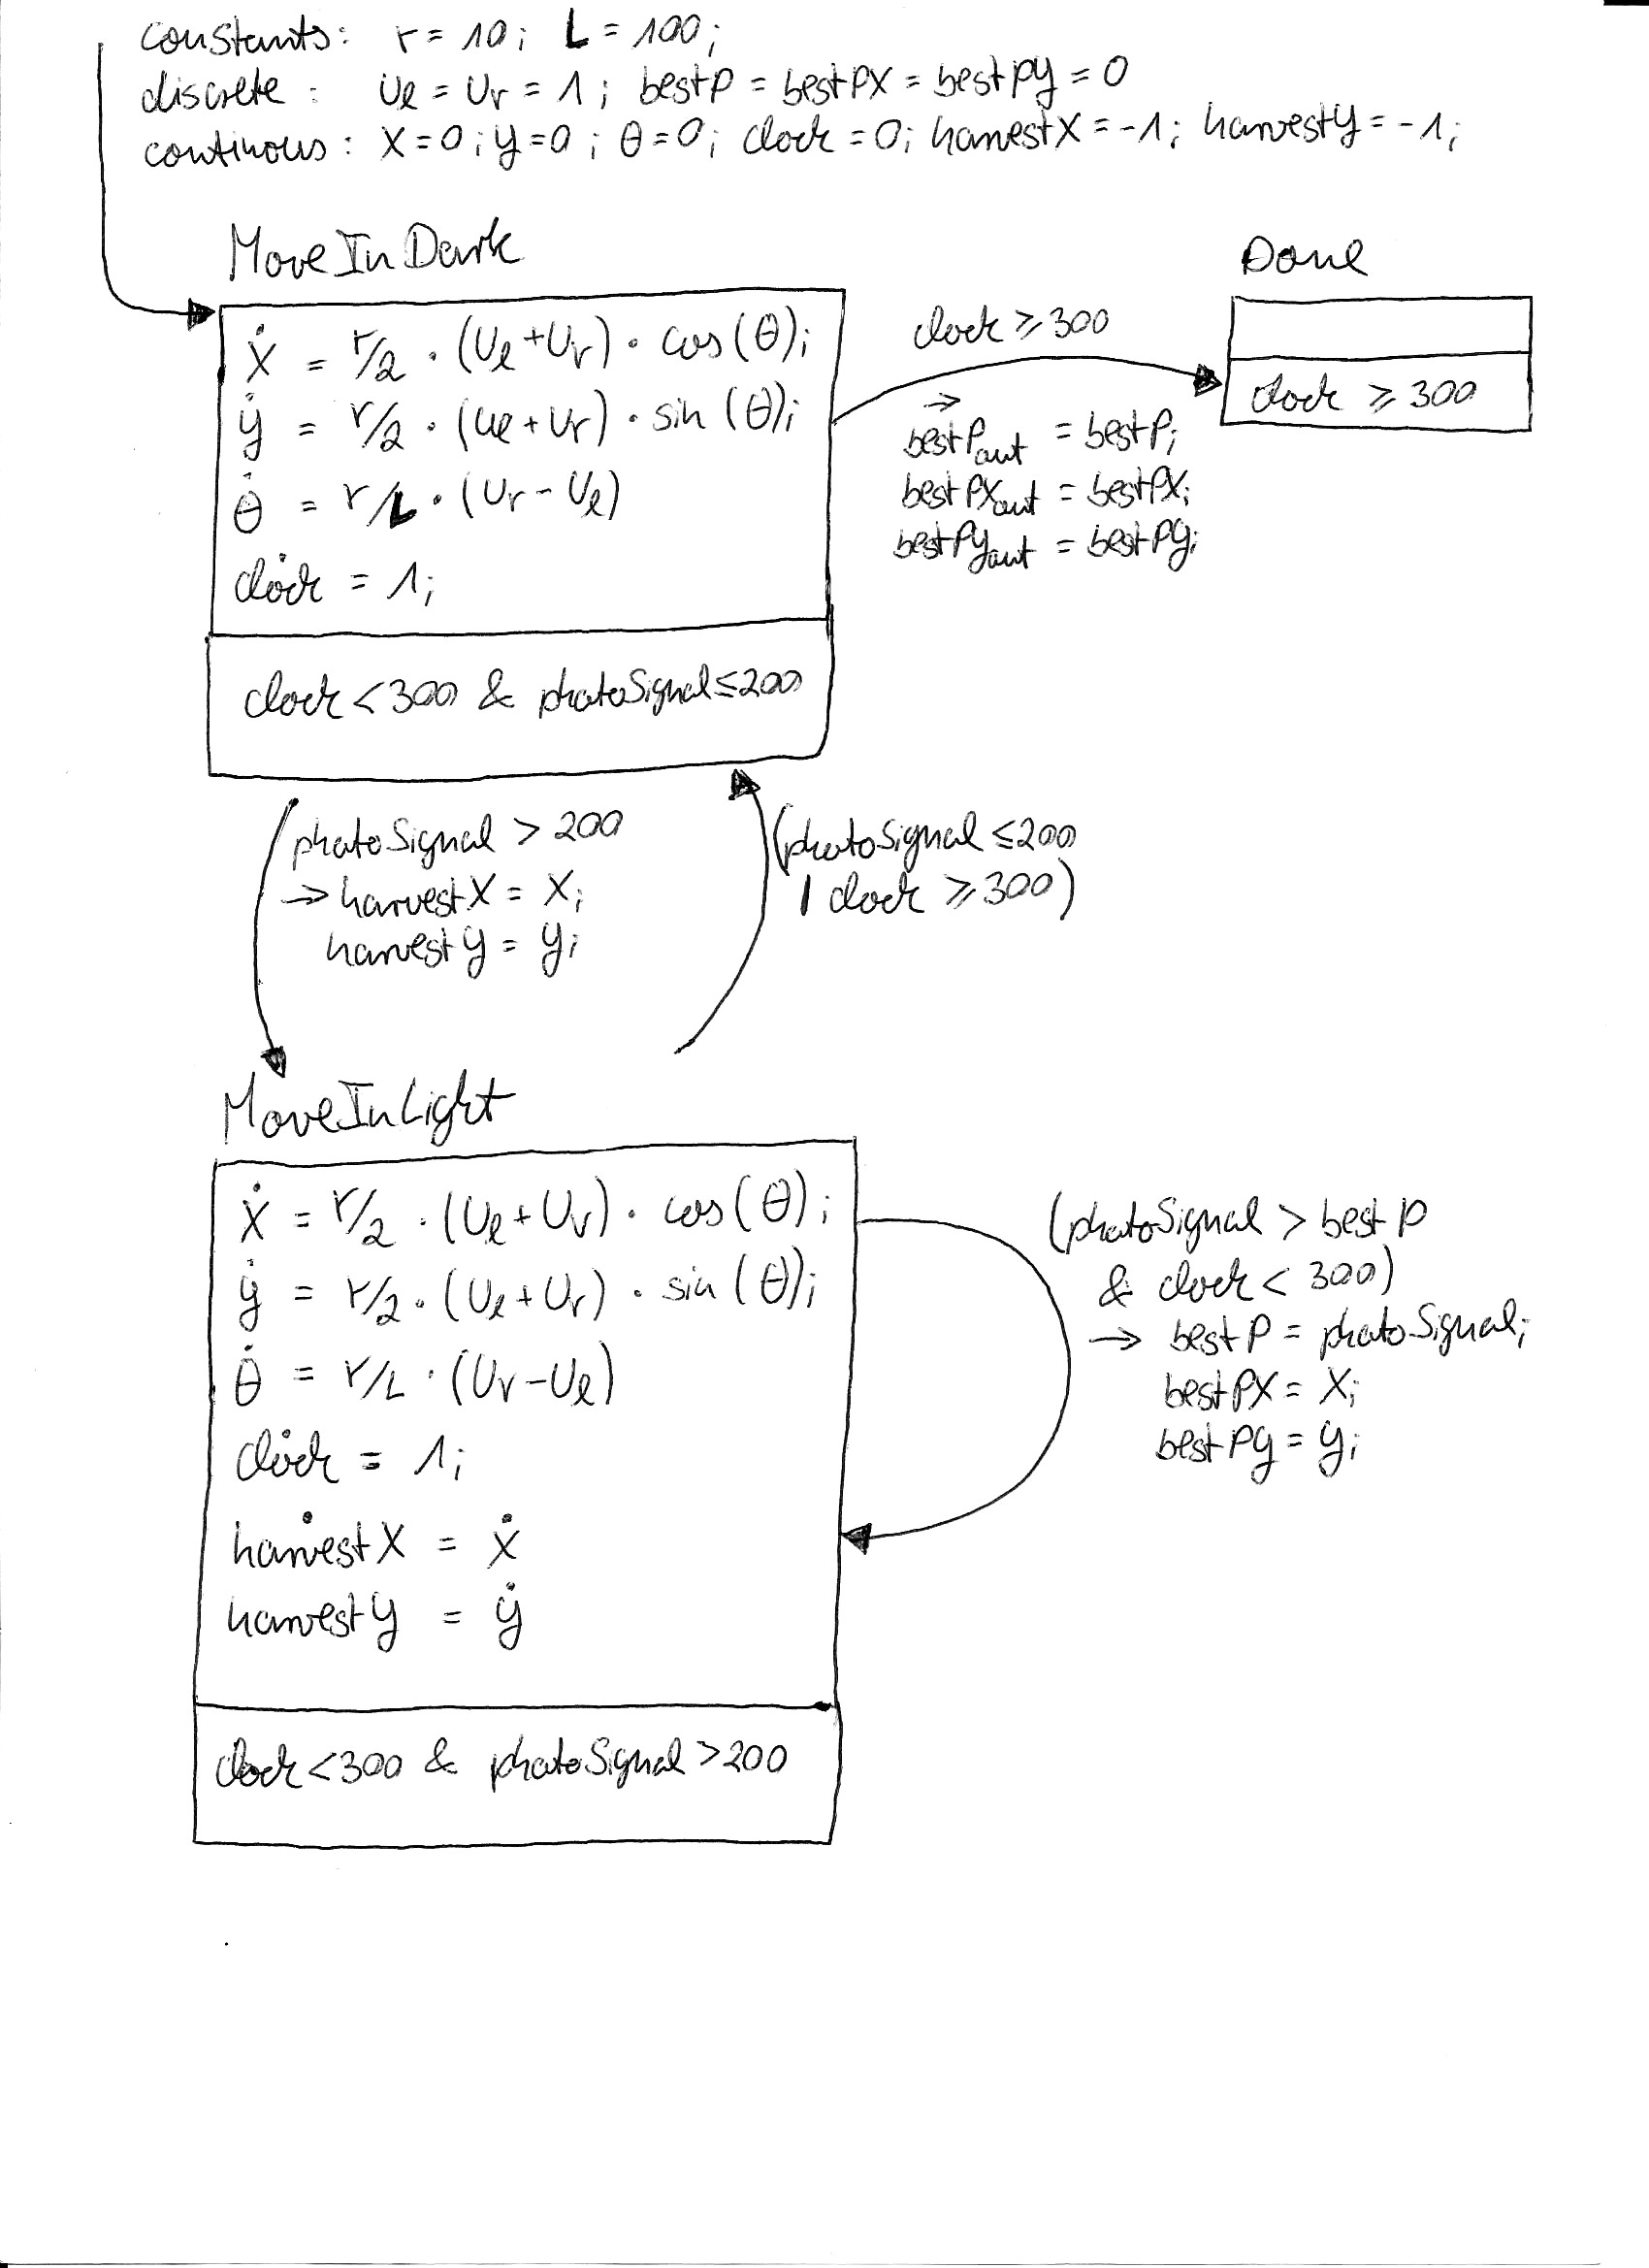
\includegraphics[scale = 0.8]{pictures/hybrid_automata_scout}

\subsection* {Collector}
The collector has two main states: Annoy and Harvest. Input are in variables harvestX and harvestY which it gets from the scout and pLeft, pFront and pRight which are the left, front and right proximity sensor readings. In the initial state Annoy, the collector drives forward and turns left or right when the proximity sensors at the sides indicate a nearby object. This is achieved by inverting the angular wheel velocitys, e.g. in order to turn left, we flip u\textsubscript{l} from 1 to -1. Just as for the scout, u\textsubscript{l} and u\textsubscript{r} are our motor control output signals. In the turning state we only have to update \Theta because the robot is not moving forward but only rotating at the same position. Once a harvest signal is received by the scout, the robot transitions to the Harvest state. There, it computes the angle to which it has to turn in order to point to the harvesting position. The function getAngle() calculates the required angle:
\begin{lstlisting}
getAngle(x, y, harvestX, harvestY) {
    vec = (harvestY- y, harvestX - x);
    angle = arctan(vec.y / vec.x);
    if (vec.x < 0) 
        angle += 180;
    if (angle > 180) 
        angle = -360 + angle;
    if (angle < -180) 
        angle = 360 - angle;
    return angle;
\end{lstlisting}
The robot compares this angle with its current angle \Theta  and transitions into either TurnLeft or TurnRight and turns until it points straight at the harvesting position. It then transitions back into the Harvest state where it moves forward towards the harvesting position. Once there, it stops. To ensure that the system does not transition back to Annoy once it has been in Harvest, we introduced the variable a that ensures that states TurnLeft and TurnRight can only transition to the states that transitioned to them and, in particular, not from Harvest to Annoy or vice versa.\\
Note that the turning functionality as we have modelled it for the collector can work int the same way for the scout. For simplicity we have omitted it in the above automaton because given the assumption from the exercise that we have an infinitely large map with no sensible boundaries it does note make a difference whether the scout makes turns or only keeps driving forward. We have modelled the automatas also in Stateflow where we let the scout make turns based on the current clock value.\\
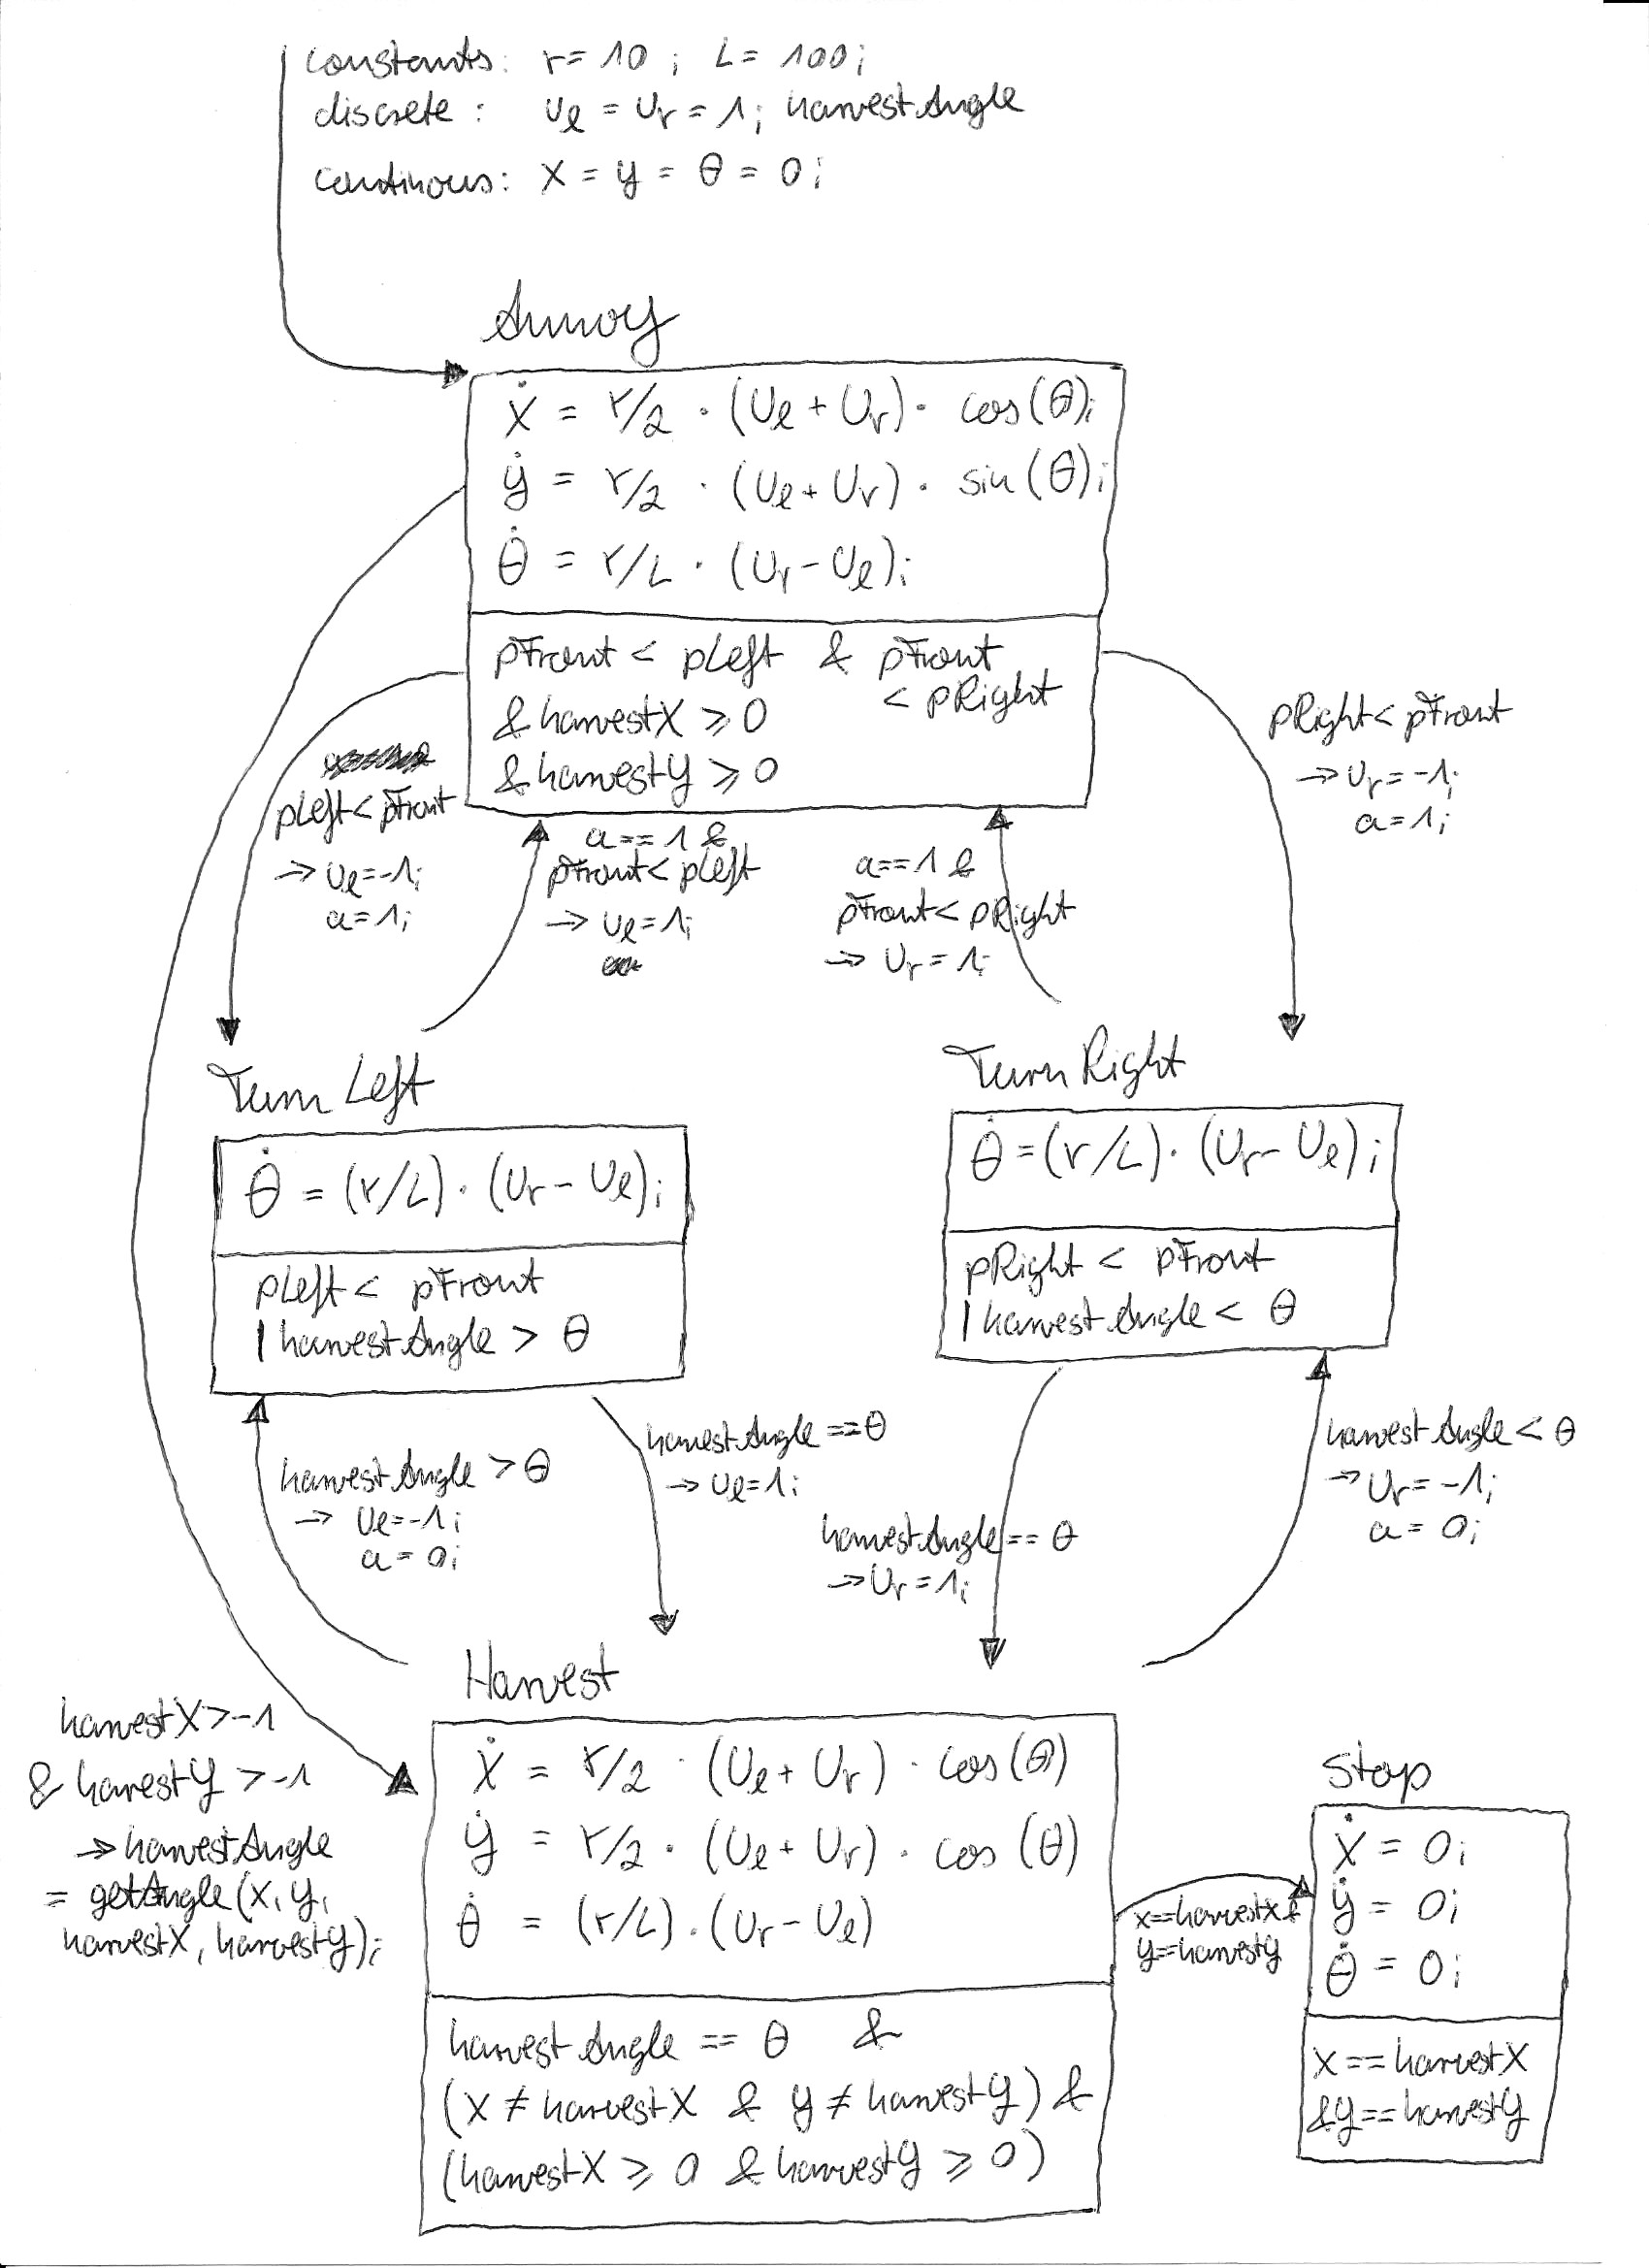
\includegraphics[scale = 0.8]{pictures/hybrid_automata_collector}

\end{document}
